% !TeX root = ../../Book2.tex
% 纲要标题：## 第17章　Morse 函数、把手与整体拓扑
% 纲要位置：几何学计划纲要.md，第 1655 行。
% 正文状态：未撰写；本文件目前是框架。

% 纲要内容开始
% 
% > 本章目标与证明范围：从非退化临界点的局部二次型，经过次水平集的真实粘合，建立 Morse 不等式与 Poincaré–Hopf。这里不把动态轨线计数当作已经建立的 Morse 同调。
% 
% 纲要内容结束

\chapter{Morse 函数、把手与整体拓扑}
\label{g2:ch:17}
\BookChapterNumber{g2:ch:17}

\begin{chapterabstract}
待撰写
\end{chapterabstract}

\begin{learninggoals}
待撰写
\end{learninggoals}

待撰写

% !TeX root = ../../Book2.tex
% 纲要标题：### 17.1 临界点及 Morse 引理
% 纲要位置：几何学计划纲要.md，第 1659 行。
% 正文状态：初稿；尚未正式审核。

% 纲要内容开始
% 
% * Hessian 的内在定义
% * 非退化标准形的逐变量消去
% * Morse 函数的存在与扰动
% * 相对及带边界数据
% 
% 纲要内容结束

\section{临界点及 Morse 引理}
\label{g2:sec:1701}

把山地浸入逐渐上涨的水中，水面经过普通高度时，岸线只是移动；经过谷底或山口时，水域可能多出一个分支，或把原有分支连接起来。对流形上的函数，决定这种变化的首先是临界点附近的形状。二阶导数给出最容易计算的信息，Morse 引理则说明：在非退化临界点附近，换一套光滑坐标就能把函数精确化成二次型。

\subsection{Hessian 的内在定义}
\label{g2:subsec:1701:01}

设 \(f:M\to\mathbb R\) 光滑。临界点 \(p\) 满足 \(\mathrm df_p=0\)，所以 \(f\) 沿任何方向的一阶变化都为零。要比较不同方向的二阶变化，不能只把某张坐标图里的二阶偏导数矩阵当成天然对象：换坐标时通常会出现额外的一阶导数项。临界点条件恰好使这些项消失。

\begin{proposition}\label{g2:prop:critical-hessian-intrinsic}
	设 \(M\) 为无边界光滑流形，\(f\in C^\infty(M)\)，\(p\) 为 \(f\) 的临界点。对 \(v,w\in\mathrm T_pM\)，任取局部光滑向量场 \(V,W\)，使 \(V_p=v\)、\(W_p=w\)，则
	\[
		\operatorname{Hess}_pf(v,w)\coloneqq V(Wf)(p)
	\]
	与延拓的选择无关，并给出 \(\mathrm T_pM\) 上的对称双线性型。在坐标 \(x^1,\ldots,x^n\) 中，它的矩阵为 \((\partial_i\partial_jf(p))\)。
\end{proposition}
\begin{proof}
	写 \(V=\sum_iV^i\partial_i\)、\(W=\sum_jW^j\partial_j\)。乘积法则给出
	\[
		V(Wf)(p)=\sum_{i,j}V^i(p)\partial_iW^j(p)\partial_jf(p)
		+\sum_{i,j}V^i(p)W^j(p)\partial_i\partial_jf(p).
	\]
	第一项因 \(\mathrm df_p=0\) 为零，第二项只取决于 \(v,w\)，并且对它们双线性。混合偏导数相等又给出对称性。定义左端用向量场作用于函数写成，已经不依赖坐标；右端给出所述矩阵。
\end{proof}

这个双线性型称为 \(f\) 在临界点的\term[Hessianxing]{Hessian 型}[Hessian]。若坐标变换写作 \(x=x(y)\)，则在临界点
\[
	H_y=J^{\mathsf T}H_xJ,\qquad J=\left(\frac{\partial x^i}{\partial y^j}(p)\right).
\]
这是合同变换。因此矩阵的秩及正、负惯性指数有坐标无关的意义；矩阵的具体特征值则随坐标缩放改变。在非临界点，\(f(x)=x\) 经过局部坐标变换 \(y=x+x^2\)，其在原点的二阶导数从 \(0\) 变成 \(-2\)。这说明临界点条件在上述构造中的作用。

\begin{definition}\label{g2:def:morse-critical-point}
	设 \(f\) 为光滑 \(n\) 维流形上的实值光滑函数，\(p\) 为内部临界点。若 \(\operatorname{Hess}_pf\) 非退化，就称 \(p\) 为\term[feituohualinjiedian]{非退化临界点}[nondegenerate critical point]。该型的负惯性指数称为 \(p\) 的\term[Morsezhibiao]{Morse 指标}[Morse index]，记作 \(\lambda(p)\)。无边界流形上的光滑函数若所有临界点都非退化，就称为\term[Morsehanshu]{Morse 函数}[Morse function]。
\end{definition}

指标 \(\lambda(p)\) 等于 Hessian 在其上负定的子空间的最大维数，满足 \(0\le\lambda(p)\le n\)。它计数的是独立的下降方向。\(x^2+y^2\)、\(-x^2+y^2\)、\(-x^2-y^2\) 在原点的指标依次为 \(0,1,2\)。其中鞍点同时有上升和下降方向，不能用“极大或极小”两类描述。

\ProseParagraphBreak

定义允许不同临界点有相同的临界值。例如 \(\cos(2\theta)\) 是圆上的 Morse 函数，却有两个同高的极大点和两个同高的极小点。以后逐个跨越临界值时，会另外使用使临界值互异的扰动。

\subsection{非退化标准形的逐变量消去}
\label{g2:subsec:1701:02}

Taylor 展开把函数写成二次项加高阶余项；对次水平集的粘合来说，精确的标准形更方便，因为可以直接沿坐标方向构造变形。下面的证明将高阶项吸收到坐标中。关键操作仍是配平方，但平方前的系数现在是光滑函数，必须同时检查所得变量确实构成坐标。

\begin{theorem}[Morse 引理]\label{g2:thm:morse-lemma}
	设 \(M\) 为无边界光滑 \(n\) 维流形，\(f:M\to\mathbb R\) 光滑，\(p\) 为指标 \(\lambda\) 的非退化临界点。则存在以 \(p\) 为原点的光滑坐标 \((y_1,\ldots,y_n)\)，使
	\begin{equation}\label{g2:eq:morse-normal-form}
		f=f(p)-y_1^2-\cdots-y_\lambda^2+y_{\lambda+1}^2+\cdots+y_n^2.
	\end{equation}
\end{theorem}
\begin{proof}
	先在以 \(p\) 为原点的小凸坐标域内计算，并减去常数 \(f(p)\)。沿线段 \(t\mapsto tx\) 两次使用微积分基本定理，利用 \(f(0)=0\)、\(\mathrm df_0=0\)，得到
	\[
		f(x)=\sum_{i,j=1}^n x_ix_j a_{ij}(x),\qquad
		a_{ij}(x)=\int_0^1(1-t)\partial_i\partial_jf(tx)\,\mathrm dt.
	\]
	矩阵 \(A(x)=(a_{ij}(x))\) 光滑、对称，且 \(A(0)=H/2\)。先作线性坐标变换，把 \(A(0)\) 化成对角矩阵；非退化性保证每个对角元非零。

	现在消去第一变量与其余变量的混合项。缩小邻域，使 \(a_{11}\) 不变号，记其符号为 \(\varepsilon_1\)。配平方得到
	\[
		f(x)=a_{11}(x)\left(x_1+\sum_{j>1}\frac{a_{1j}(x)}{a_{11}(x)}x_j\right)^2
		+\sum_{i,j>1}x_ix_j\left(a_{ij}(x)-\frac{a_{i1}(x)a_{1j}(x)}{a_{11}(x)}\right).
	\]
	令
	\[
		y_1=\sqrt{|a_{11}(x)|}\left(x_1+\sum_{j>1}\frac{a_{1j}(x)}{a_{11}(x)}x_j\right),
		\qquad y_j=x_j\quad(j>1).
	\]
	由于 \(a_{1j}(0)=0\) 对 \(j>1\) 成立，此变换在零处的微分是对角矩阵，第一对角元为 \(\sqrt{|a_{11}(0)|}\)，其余为 \(1\)。第一卷第11章第3节的逆函数定理因而给出局部光滑逆。换成这套坐标后，函数成为
	\[
		\varepsilon_1y_1^2+\sum_{i,j>1}y_iy_j b_{ij}(y),
	\]
	其中 \(B(0)\) 仍是非退化对角矩阵。这里 \(b_{ij}\) 可以依赖 \(y_1\)，并不影响下一步：保持 \(y_1\) 不动，对其余变量配平方即可。

	更一般地，已分离出前 \(k-1\) 个平方后，余项具有 \(\sum_{i,j\ge k}z_iz_j c_{ij}(z)\) 的形式，且剩余系数矩阵在零处非退化、对角。保持前 \(k-1\) 个坐标和后 \(n-k\) 个坐标不动，只把第 \(k\) 个坐标改成
	\[
		\sqrt{|c_{kk}(z)|}\left(z_k+\sum_{j>k}\frac{c_{kj}(z)}{c_{kk}(z)}z_j\right).
	\]
	同一微分检验保证这仍是坐标变换，并分离出一个符号为 \(\operatorname{sgn}c_{kk}(0)\) 的平方。有限次之后得到 \(f=\sum_i\varepsilon_i y_i^2\)。这套坐标中的 Hessian 为 \(2\operatorname{diag}(\varepsilon_1,\ldots,\varepsilon_n)\)，合同不变性说明负号恰有 \(\lambda\) 个。重排坐标并加回 \(f(p)\)，即得公式。
\end{proof}

在标准形中，微分为 \(2\sum_i\varepsilon_i y_i\,\mathrm dy_i\)，所以原点是邻域内唯一的临界点。非退化临界点因此孤立；紧流形上的 Morse 函数只有有限个临界点，因为临界点集是闭的，而这些隔离邻域给出它的一个开覆盖，紧性提供有限子覆盖。

\begin{example}\label{g2:exm:morse-coordinate-completion}
	考虑 \(f(x,y)=x^2+2xy+2y^2+y^3\)。原点的 Hessian 为 \(\left(\begin{smallmatrix}2&2\\2&4\end{smallmatrix}\right)\)，正定。直接写成
	\[
		f=(x+y)^2+y^2(1+y)
	\]
	后，取 \(u=x+y\)、\(v=y\sqrt{1+y}\)，便得到 \(f=u^2+v^2\)。变换在原点的行列式为 \(1\)，所以 \((u,v)\) 确为局部坐标。余项 \(y^3\) 进入了坐标 \(v\)，无须令它等于零或用近似舍去。
\end{example}

退化临界点可能有不同的局部行为。\(x^4+y^2\) 在原点是严格极小值，但 Hessian 有核；任何局部坐标变换都保持 Hessian 的秩，故它不能变成非退化二次型。非退化性给出了能被有限个正、负平方完全描述的那类临界点。

\subsection{Morse 函数的存在与扰动}
\label{g2:subsec:1701:03}

局部标准形很有用，还需要知道流形上能否找到这样的函数。把 \(\mathrm df\) 看成余切丛的一个截面，临界点就是它与零截面的交点。在临界点，截面沿纤维方向的导数正是 Hessian，所以非退化性等价于这个交点横截。扰动时须仍保持截面是某个函数的微分；直接对函数加入局部线性项就能做到这一点。

\begin{theorem}\label{g2:thm:morse-approximation}
	设 \(M\) 为有限维、Hausdorff、第二可数的无边界光滑流形，\(r\ge2\) 为有限整数。每个 \(f\in C^\infty(M)\) 的任意强 \(C^r\) 邻域中都有光滑 Morse 函数。若 \(M\) 紧，则 Morse 函数还构成 \(C^\infty(M)\) 中关于 \(C^2\) 拓扑的开集。
\end{theorem}
\begin{proof}
	先说明局部扰动。在坐标域 \(U\) 中取紧集 \(K\)，并选紧支于 \(U\) 的光滑函数 \(\rho\)，使其在 \(K\) 的一个邻域 \(V\) 上等于 \(1\)。令
	\[
		f_a=f+\rho\sum_{j=1}^n a_jx^j,\qquad a\in\mathbb R^n,
	\]
	并在 \(U\) 外仍取 \(f_a=f\)。在 \(V\) 上，微分的坐标分量为
	\[
		G(a,x)=(\partial_1f(x)+a_1,\ldots,\partial_nf(x)+a_n).
	\]
	\(G\) 关于参数的微分为恒等矩阵，所以它是淹没。\cref{g2:thm:parametric-transversality}说明：任意小参数中都有 \(a\)，使 \(G_a\) 横截于 \(\{0\}\)。在 \(G_a=0\) 处，\(\mathrm D_xG_a\) 就是 \(f_a\) 的 Hessian，横截等价于它可逆。因此 \(f_a\) 在 \(K\) 上只有非退化临界点，且扰动在任意指定有限阶意义下随 \(a\to0\) 趋于零。

	保持已经得到的非退化性需要二阶控制。对任意紧集 \(L\)，条件“\(f\) 在 \(L\) 上的全部临界点非退化”等价于微分截面 \(x\mapsto(x,\mathrm df_x)\) 在 \(L\) 上横截于余切丛的零截面。后者是闭嵌入子流形。由\cref{g2:prop:transversality-open-on-compact}，该条件对截面的 \(C^1\) 小扰动开放，也就对函数的 \(C^2\) 小扰动开放。坐标上，这分别控制非临界区域的一阶导数不变成零，以及临界点邻域内 Hessian 的可逆性。

	若 \(M\) 紧，取有限个上述紧集 \(K_i\)，使其内部覆盖 \(M\)，依次作局部扰动。在每一步把参数取得足够小，就能保留先前紧集上的非退化性，并使总 \(C^r\) 误差小于给定界。最后的函数在所有 \(K_i\) 上满足条件，因而为 Morse 函数。刚才的紧集开放性取 \(L=M\)，也证明了紧情形的开放结论。

	一般的 \(M\) 取可数、局部有限的相对紧坐标域 \(U_i\)，以及 \(K_i\subset U_i\)，使 \(\operatorname{Int}K_i\) 覆盖 \(M\)。每步扰动紧支于 \(U_i\)。对原强邻域在第 \(\ell\) 个控制块上的容差 \(\varepsilon_\ell\)，要求第 \(i\) 步在那里耗用小于 \(2^{-i-1}\varepsilon_\ell\)。第 \(i\) 步完成后，在 \(K_i\) 上选一个保持非退化性的 \(C^2\) 容差 \(\delta_i>0\)；对后来第 \(j\) 步，另要求它在覆盖 \(K_i\) 的坐标块上的 \(C^2\) 改变量小于 \(2^{-(j-i+1)}\delta_i\)。每步只遇到有限多个原控制块和有限多个先前要求，故可以同时满足。局部有限性又使每点附近只有有限次实际改变，所以极限函数光滑。误差级数保证它仍在原邻域内，并保留每个 \(K_i\) 上的非退化性。这是\cref{g2:thm:relative-transversality}证明中的逐块选择，此处每一步都通过函数的局部线性项实施。
\end{proof}

\begin{proposition}\label{g2:prop:distinct-morse-critical-values}
	设 \(M\) 为紧无边界光滑流形，\(f:M\to\mathbb R\) 为 Morse 函数。任意有限阶 \(C^r\) 邻域内都存在 Morse 函数 \(g\)，与 \(f\) 有完全相同的临界点和指标，且不同临界点的 \(g\) 值互异。
\end{proposition}
\begin{proof}
	临界点为有限个 \(p_1,\ldots,p_N\)。取两两不交的坐标邻域 \(U_i\)，以及紧支于 \(U_i\)、在 \(p_i\) 的较小邻域 \(V_i\) 上为 \(1\) 的截断函数 \(\rho_i\)。令 \(g=f+\sum_i c_i\rho_i\)。在每个 \(V_i\) 上，\(g\) 与 \(f\) 相差常数，故临界点和 Hessian 完全相同。在紧集 \(M\setminus\bigcup_iV_i\) 上，\(\mathrm df\) 处处不为零；相对于任一度量，它的范数有正下界。令全部 \(c_i\) 足够小，便使这里的 \(\mathrm dg\) 仍不为零。最后避开有限个等式 \(f(p_i)+c_i=f(p_j)+c_j\)，可使所有临界值互异。参数还可任意小，所以满足所给 \(C^r\) 要求。
\end{proof}

这种调整改变临界高度，却不改变局部的下降方向数。它使相邻两个正则水平之间可以只放一个临界点，正适合下一节逐次描述次水平集的变化。

\subsection{相对及带边界数据}
\label{g2:subsec:1701:04}

在粘合问题中，一部分函数已经规定好，例如边界附近要把高度直接当成领圈参数。此时扰动应避开那一部分。能保持哪些数据，取决于固定区域里原有临界点是否已经非退化。

\begin{proposition}\label{g2:prop:relative-morse-approximation}
	设 \(M\) 为有限维、Hausdorff、第二可数的无边界光滑流形，\(A\subset M\) 闭，\(f\in C^\infty(M)\) 在 \(A\) 的某开邻域上只有非退化临界点。则对任意有限整数 \(r\ge2\)，可在 \(f\) 的任意强 \(C^r\) 邻域内找到 Morse 函数 \(g\)，使 \(g=f\) 在 \(A\) 的某开邻域上成立。
\end{proposition}
\begin{proof}
	在已满足条件的开集 \(U\) 中选 \(A\subset W\subset\overline W\subset V\subset\overline V\subset U\)。先用逐紧块的 \(C^2\) 开放性，缩小给定强邻域，使其中的函数在 \(\overline V\) 上都保持非退化性。再对 \(M\setminus V\) 取局部有限的紧坐标块及支集域，使支集均避开 \(\overline W\)。按\cref{g2:thm:morse-approximation}的局部线性扰动及误差分配逐块处理，得到在整个 \(M\) 上为 Morse 的 \(g\)。全部改动支集避开 \(\overline W\)，所以 \(g=f\) 于 \(W\)。
\end{proof}

带边界时，本章所用数据是边界为正则水平，临界点都在内部。下述构造同时适用于只有外边界的紧流形和两端高度已指定的配边。

\begin{proposition}\label{g2:prop:boundary-morse-function}
	设 \(M\) 为紧光滑带边界 \(n\) 维流形，\(n\ge1\)，并把边界分成互不相交的开闭子集 \(\partial M=\partial_-M\amalg\partial_+M\)，允许其中一部分为空。给定 \(a<b\)，存在光滑函数 \(f:M\to[a,b]\) 及两侧的领圈，使
	\[
		f(x,t)=a+t\quad\text{在 }\partial_-M\text{ 的较小领圈内},\qquad
		f(x,t)=b-t\quad\text{在 }\partial_+M\text{ 的较小领圈内}.
	\]
	这里 \(t\ge0\) 指向内部。函数在内部取值于 \((a,b)\)，所有临界点非退化且临界值互异。可选择在领圈内为 \(\mathrm dt^2+g_{\partial M}\) 的 Riemann 度量；此时 \(\nabla f\) 在 \(\partial_-M\) 严格向内，在 \(\partial_+M\) 严格向外。
\end{proposition}
\begin{proof}
	由\cref{g2:thm:collar-neighborhood}选择两侧互不相交的领圈，并把宽度取得小于 \((b-a)/4\)。在更小的领圈内分别规定 \(f_0=a+t\)、\(f_0=b-t\)，在领圈以外取常数 \((a+b)/2\)。用只依赖 \(t\) 的截断函数把这些表达作凸组合，得到光滑 \(f_0\)。在内部出现的各个参与值都严格介于 \(a,b\)，所以 \(a<f_0<b\)；在固定的较小领圈内，\(\mathrm df_0=\pm\mathrm dt\)，没有临界点。

	对 \(\operatorname{Int}M\) 应用\cref{g2:prop:relative-morse-approximation}，固定一条更窄领圈中的全部函数值。所有实际改动可支撑在远离边界的一个紧集内；在那里 \(f_0\) 与 \(a,b\) 都有正距离。因此同时要求 \(C^0\) 误差足够小，就能保持 \(a<f<b\)。所得函数与 \(f_0\) 在边界邻域一致，故光滑延拓到 \(M\)。临界点避开固定领圈，处在紧集内，因而只有有限个。按\cref{g2:prop:distinct-morse-critical-values}的截断常数构造，在内部各临界点附近作更小的扰动，即可使临界值互异而不改变边界数据及值域。

	在领圈上先取乘积度量 \(\mathrm dt^2+g_{\partial M}\)，再用单位分解延拓为全局正定度量，并保持较小领圈上的度量不变。由梯度定义 \(g(\nabla f,\cdot)=\mathrm df\)，两端分别有 \(\nabla f=\partial_t\) 和 \(\nabla f=-\partial_t\)。因为 \(t\) 向内增加，这给出所需指向。
\end{proof}

特别地，取 \(\partial_-M=\varnothing\)，便得到边界为最高水平、梯度处处外向的 Morse 函数。它将用于带边界的 Poincaré--Hopf 公式。若事先要求在某邻域逐点保留一个退化临界点，Morse 逼近就无法满足；相对命题中的条件准确描述了固定数据应先具备的性质。

% !TeX root = ../../Book2.tex
% 纲要标题：### 17.2 次水平集的变化
% 纲要位置：几何学计划纲要.md，第 1666 行。
% 正文状态：初稿；尚未正式审核。

% 纲要内容开始
% 
% * 无临界区间的梯度变形
% * 跨越单个临界值的局部模型
% * 把手附着映射与指标
% * 从把手到胞腔同伦类型
% 
% 纲要内容结束

\section{次水平集的变化}
\label{g2:sec:1702}

把一个函数的高度从低向高扫描，得到一族不断增大的区域。Morse 引理描述了临界点附近的高度，却还没有说明这个小区域怎样接到已经出现的部分。本节把两件事连接起来：无临界点处用流搬运等高面，临界点附近则直接放入一个有厚度的圆盘。它的厚度保留光滑流形结构，中心圆盘负责改变同伦型。

\subsection{无临界区间的梯度变形}
\label{g2:subsec:1702:01}
记 \(M^a=f^{-1}(( -\infty,a])\)，称为 \(f\) 的\term[cishuipingji]{次水平集}[sublevel set]。若 \(a\) 是正则值且 \(f^{-1}(a)\) 位于 \(M\) 内部，则正则水平集定理给出 \(M^a\) 的新边界 \(f^{-1}(a)\)。在局部坐标中，\(f-a\) 本身就是横向坐标，因而次水平条件成为一个半空间条件。

\begin{proposition}\label{g2:prop:morse-regular-band}
	设 \(M\) 为光滑流形，\(f:M\to\mathbb R\) 光滑，\(a<b\)，且 \(f^{-1}([a,b])\) 是位于 \(M\) 内部的紧集，其中没有临界点。则
	\[
		f^{-1}([a,b])\cong f^{-1}(a)\times[a,b]
	\]
	的微分同胚可取为使 \(f\) 对应第二投影；\(M^a\hookrightarrow M^b\) 是强形变收缩的包含映射，\(M^a\) 与 \(M^b\) 也微分同胚。
\end{proposition}
\begin{proof}
	选光滑 Riemann 度量。由于 \(\mathrm{d}f\ne0\)，向量场
	\[
		Y=\frac{\operatorname{grad}f}{|\operatorname{grad}f|^2}
	\]
	在闭带的某邻域有定义，且 \(Yf=1\)。用紧支截断将它延拓到 \(M\) 上，保持闭带附近的表达。第一卷第13章第1节的光滑流定理及第2节的紧支完备性说明，这个紧支向量场的流 \(\Phi_t\) 对全部时间存在；轨道留在闭带期间满足 \(f(\Phi_t(x))=f(x)+t\)。于是
	\[
		(z,t)\longmapsto\Phi_{t-a}(z),\qquad
		x\longmapsto\bigl(\Phi_{a-f(x)}(x),f(x)\bigr)
	\]
	互为光滑逆。这也解释了紧性的作用：所需时间内的轨道不会在空间中逃走。

	在 \(M^b\) 上令
	\[
		R_s(x)=
		\begin{cases}
			x,&f(x)\le a,\\
			\Phi_{-s(f(x)-a)}(x),&a\le f(x)\le b,
		\end{cases}
		\qquad 0\le s\le1.
	\]
	两式在 \(f=a\) 处一致，给出连续同伦，且逐点固定 \(M^a\)。当 \(s=1\) 时，整个上方闭带落到 \(f^{-1}(a)\)，故得到强形变收缩。

	为得到微分同胚，取 \(a\) 以下一个足够薄的无临界领带；它由闭带的紧性及 \(\mathrm{d}f\ne0\) 延伸得到。在乘积坐标中，用一个光滑严格递增的区间微分同胚把 \([a-\delta,b]\) 压到 \([a-\delta,a]\)，并使它在左端附近为恒等。与更低处的恒等映射拼接，即得 \(M^b\cong M^a\)。这里的压缩移动了边界；前一个强形变收缩则只要求连续，并固定整个旧区域。
\end{proof}

\begin{example}
	在 \(M=\mathbb R^2\setminus\{(0,0)\}\) 上取 \(f(x,y)=x\)。它处处无临界点，但 \(f^{-1}(0)\) 有两个连通分支，其他水平集都是一条直线。\(M^{-1}\) 可缩，而 \(M^1\) 绕缺失的原点有一个不可缩圆周。闭带不紧，正是上面命题无法使用的条件：穿过原点的水平搬运会离开 \(M\)。
\end{example}

\subsection{跨越单个临界值的局部模型}
\label{g2:subsec:1702:02}
现在设临界点 \(p\) 的指标为 \(\lambda\)，写 \(\mu=n-\lambda\)。由\cref{g2:thm:morse-lemma}，可在 \(p\) 附近选坐标 \((u,v)\in\mathbb R^\lambda\times\mathbb R^\mu\)，使
\begin{equation}\label{g2:eq:morse-local-handle-model}
	f(u,v)=c-|u|^2+|v|^2,\qquad c=f(p).
\end{equation}
负方向 \(u\) 在离开临界点时降低高度，正方向 \(v\) 提供横向厚度。选充分小的 \(\varepsilon>0\) 和 \(r>0\)，满足 \(r^2<\varepsilon\)，并使下面的闭集全落在坐标域中：
\[
	H=\bigl\{(u,v):|v|\le r,\ |u|^2\le\varepsilon+|v|^2\bigr\}.
\]
它有一个明确的乘积参数化
\begin{equation}\label{g2:eq:morse-handle-parametrization}
	\Phi:D^\lambda\times D^\mu\longrightarrow H,
	\qquad
	\Phi(x,w)=\bigl(\sqrt{\varepsilon+r^2|w|^2}\,x,rw\bigr).
\end{equation}
缩放因子严格为正，故这是带角流形之间的微分同胚。代入高度可见
\[
	f\circ\Phi
	=c+r^2|w|^2-(\varepsilon+r^2|w|^2)|x|^2.
\]
因此 \(H\subset M^{c+\varepsilon}\)，且
\begin{equation}\label{g2:eq:morse-handle-attaching-face}
	H\cap M^{c-\varepsilon}
	=\Phi(S^{\lambda-1}\times D^\mu)
	\subset f^{-1}(c-\varepsilon).
\end{equation}
新块只沿第一因子的边界贴到旧区域上；它的其余内部点都在旧水平以上。\(\lambda=0\) 时约定 \(S^{-1}=\varnothing\)，新块与旧区域不相交；\(\mu=0\) 时新块是整个 \(n\) 维圆盘，其全部边界都被附着。

\begin{figure}[htbp]
	\centering
	% !TeX root = ../Book2.tex
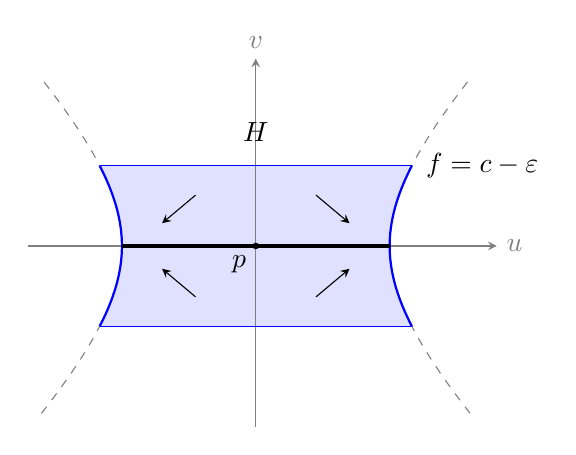
\begin{tikzpicture}[scale=1.7,>=stealth]
	\fill[blue!12] plot[domain=-.6:.6,samples=40] ({sqrt(1+\x*\x)},\x) -- plot[domain=.6:-.6,samples=40] ({-sqrt(1+\x*\x)},\x) -- cycle;
	\draw[->,gray] (-1.7,0)--(1.8,0) node[right] {\(u\)};
	\draw[->,gray] (0,-1.35)--(0,1.4) node[above] {\(v\)};
	\draw[dashed,gray] plot[domain=-1.25:1.25,samples=50] ({sqrt(1+\x*\x)},\x);
	\draw[dashed,gray] plot[domain=-1.25:1.25,samples=50] ({-sqrt(1+\x*\x)},\x);
	\draw[thick,blue] plot[domain=-.6:.6,samples=40] ({sqrt(1+\x*\x)},\x);
	\draw[thick,blue] plot[domain=-.6:.6,samples=40] ({-sqrt(1+\x*\x)},\x);
	\draw[blue] ({-sqrt(1.36)},.6)--({sqrt(1.36)},.6);
	\draw[blue] ({-sqrt(1.36)},-.6)--({sqrt(1.36)},-.6);
	\draw[very thick] (-1,0)--(1,0);
	\draw[->] (.45,.38)--(.7,.17);
	\draw[->] (-.45,.38)--(-.7,.17);
	\draw[->] (.45,-.38)--(.7,-.17);
	\draw[->] (-.45,-.38)--(-.7,-.17);
	\fill (0,0) circle (.025) node[below left] {\(p\)};
	\node at (0,.85) {\(H\)};
	\node[anchor=west] at (1.2,.6) {\(f=c-\varepsilon\)};
\end{tikzpicture}

	\caption[临界点附近的把手]{二维指标一模型 \(f-c=-u^2+v^2\)。阴影块 \(H\) 沿左右两段粗曲线贴到旧次水平集；中心线是核心圆盘。下降向量场沿 \(u\) 方向向外、沿 \(v\) 方向向内，将剩余闭带送入旧区域与新块的并。}
	\label{g2:fig:morse-local-handle}
\end{figure}

局部二次型还提供了控制剩余空间的向量场。在这个坐标域内选 Euclid 度量，则负梯度为
\[
	X=(2u,-2v),\qquad Xf=-4(|u|^2+|v|^2).
\]
在自由面 \(|v|=r\) 上，有 \(X(|v|^2-r^2)=-4r^2<0\)，所以流从外面进入 \(H\)；在旧水平 \(f=c-\varepsilon\) 上，它也严格指向旧次水平集。除原点外，高度一直下降。这两个明确的不等式将局部模型与整体流联系起来。

\subsection{把手附着映射与指标}
\label{g2:subsec:1702:03}
\begin{definition}\label{g2:def:morse-handle}
	设 \(W\) 为光滑 \(n\) 维带边界流形，\(0\le\lambda\le n\)。一个\term[bashou]{指标 \(\lambda\) 的把手}[handle of index \(\lambda\)]是乘积 \(D^\lambda\times D^{n-\lambda}\)，其附着面为 \(S^{\lambda-1}\times D^{n-\lambda}\)。给定光滑嵌入
	\[
		\varphi:S^{\lambda-1}\times D^{n-\lambda}\longrightarrow\partial W,
	\]
	将附着面上的点 \((x,w)\) 与 \(\varphi(x,w)\) 识别，再将接缝的角磨圆，称为向 \(W\) 附着这个把手。\(D^\lambda\times\{0\}\) 称为\term[hexinyuanpan]{核心圆盘}[core disk]，\(\{0\}\times D^{n-\lambda}\) 称为\term[gonghexinyuanpan]{共核心圆盘}[cocore disk]。
\end{definition}

附着数据包含整个有厚度的球面邻域。仅指定中心球面 \(S^{\lambda-1}\times\{0\}\) 的像，还没有说明横向圆盘怎样放置；后续手术中的法标架正来自这份数据。

\begin{theorem}[Morse 把手附着定理]\label{g2:thm:morse-handle-attachment}
	设 \(M\) 为光滑 \(n\) 维流形，\(f:M\to\mathbb R\) 光滑，\(a<b\) 为正则值，且紧闭带 \(f^{-1}([a,b])\) 位于 \(M\) 内部。若其中恰有一个临界点 \(p\)，该点非退化且指标为 \(\lambda\)，则 \(M^b\) 微分同胚于向 \(M^a\) 附着一个指标 \(\lambda\) 的把手并磨圆所得的流形。附着映射可由式\eqref{g2:eq:morse-handle-parametrization}的附着面沿无临界带下降到 \(f^{-1}(a)\) 得到。
\end{theorem}
\begin{proof}
	令 \(c=f(p)\)。先取充分小的 \(\varepsilon>0\)，使 \(a<c-\varepsilon<c+\varepsilon<b\)，并能使用上面的坐标块。两侧闭带 \([a,c-\varepsilon]\)、\([c+\varepsilon,b]\) 都没有临界点，\cref{g2:prop:morse-regular-band}将它们识别为领带。因此只需处理 \(a=c-\varepsilon\)、\(b=c+\varepsilon\)；最后把附着映射沿下方的流搬回原来的水平即可。

	记 \(A=M^{c-\varepsilon}\)，取式\eqref{g2:eq:morse-handle-parametrization}中的 \(H\)，令 \(K=A\cup H\)。式\eqref{g2:eq:morse-handle-attaching-face}说明，\(K\) 确实是沿嵌入 \(\Phi|_{S^{\lambda-1}\times D^\mu}\) 作出的把手附着商：两块的交恰为附着面，且 \(H\) 紧，故这个商到它们在 \(M\) 中的并是同胚。坐标参数化给出了新块的光滑结构。

	将局部 Euclid 度量与外部任意度量用单位分解拼接，使其在 \(H\) 的一个邻域内仍为 Euclid 度量。令 \(X=-\operatorname{grad}f\)。旧边界上 \(Xf<0\)，新块的自由面上 \(X(|v|^2-r^2)<0\)，所以 \(X\) 在 \(K\) 的每个边界面都朝向内部。它的唯一零点 \(p\) 已在 \(K\) 内部。

	先把交界的角变成光滑边界。若 \(0<\lambda<n\)，角附近可用两个独立的横向函数
	\[
		s=f-c+\varepsilon,\qquad t=|v|^2-r^2
	\]
	描述 \(K=\{s\le0\}\cup\{t\le0\}\)。两者的微分在 \(s=t=0\) 处线性无关：此处 \(u,v\) 均非零，而 \(\mathrm{d}t\) 没有 \(u\) 分量。取光滑偶函数 \(\eta_\delta\)，满足 \(\eta_\delta(z)\ge|z|\)、\(|\eta_\delta'(z)|\le1\)，并在 \(|z|\ge\delta\) 时等于 \(|z|\)。例如将绝对值与支集很小的偶非负平滑核卷积即可。把角附近的边界换成
	\[
		m_\delta(s,t)=\frac{s+t-\eta_\delta(s-t)}2=0,
	\]
	并取 \(m_\delta\le0\) 一侧。它包含原来的 \(K\)，且新增边界只发生在 \(|s|,|t|\) 都很小的地方，因此与角邻域外的原边界精确拼接。两偏导非负且之和为一；由于 \(Xs<0\)、\(Xt<0\)，有 \(Xm_\delta<0\)，所以新边界光滑，\(X\) 仍严格朝内。记磨圆后的区域为 \(K_\delta\)。取 \(\delta\) 小，可使 \(K_\delta\setminus A\subset\{f<c+\varepsilon\}\)。指标为 \(0\) 或 \(n\) 时没有这种角，直接令 \(K_\delta=K\)。

	剩下的紧区域 \(M^{c+\varepsilon}\setminus\operatorname{int}_M K_\delta\) 没有临界点。其上 \(|\operatorname{grad}f|^2\) 有严格正的下界。因此从新增边界 \(B=\partial K_\delta\cap f^{-1}([c-\varepsilon,c+\varepsilon])\) 沿 \(-X\) 向外运动，必在有限时间到达 \(f=c+\varepsilon\)：若一直不到达，高度将以一个固定正速度增加而始终不超过该值，矛盾。反向轨道同样在有限时间到达 \(B\)。光滑依赖与隐函数定理说明首次到达时间 \(\tau(z)>0\) 随 \(z\in B\) 光滑变化，因为两端的向量场都横截边界。流遂给出
	\[
		M^{c+\varepsilon}\setminus\operatorname{int}_M K_\delta
		\cong\{(z,t):z\in B,\ 0\le t\le\tau(z)\}.
	\]
	没有外部边界的连通分支已完全包含于 \(K_\delta\)，在此乘积中不出现。

	这段外部乘积可以吸收到 \(K_\delta\) 的一个内部领圈中。具体说，在每条领线的区间 \([-h,\tau(z)]\) 上，选依赖 \(z\) 光滑、在左端附近恒等的严格递增微分同胚到 \([-h,0]\)；\(B\) 紧，故可统一取 \(h>0\)。这样的区间映射可由一个处处为正、左端等于一的光滑密度积分而成，再使总积分等于 \(h\)。与领圈外的恒等映射拼接，得到 \(M^{c+\varepsilon}\cong K_\delta\)。至此既确定了附着面，也处理了剩余空间和接缝光滑结构。
\end{proof}

上面证明还给出一个相对结论，后面计算同调时会用到：未磨圆的 \(K=A\cup H\) 是 \(M^{c+\varepsilon}\) 的强形变收缩像。沿 \(X\) 流到第一次进入 \(K\) 即停下，进入时间在各光滑面附近由横截性连续变化；角附近它是到两个边界面的时间的较小者，仍连续。剩余紧区域中 \(Xf\) 有严格负的上界，保证每条轨道都在有限时间进入。将这段时间乘以同伦参数，就得到固定 \(K\)、从而固定 \(A\) 的收缩。这个结论不需要先磨圆。

\ProseParagraphBreak

在曲面上，指标零把手是一个新圆盘；指标一把手是沿两条短边接上的带；指标二把手沿整个圆周填入一个圆盘。中间那条带可能连接两个原有分支，也可能把同一个分支的两个部位连起来。局部指标决定新增块的形状，附着位置则决定全局拓扑怎样改变。

\subsection{从把手到胞腔同伦类型}
\label{g2:subsec:1702:04}
把手中 \(D^{n-\lambda}\) 的厚度可以连续压掉，但在压缩时必须固定已经贴在旧区域上的整个附着面。直接将 \((x,w)\) 送到 \((x,(1-s)w)\) 会移动附着面，无法与旧区域上的恒等映射拼接。下面给出保持粘合位置的收缩。

\begin{lemma}\label{g2:lem:handle-core-retraction}
	乘积圆盘 \(D^\lambda\times D^\mu\) 强形变收缩到
	\[
		Q=(D^\lambda\times\{0\})\cup(S^{\lambda-1}\times D^\mu).
	\]
	因此沿 \(\varphi\) 附着把手所得的空间强形变收缩到沿 \(\varphi(x,0)\) 附着核心 \(D^\lambda\) 所得的空间，且收缩固定旧空间。
\end{lemma}
\begin{proof}
	给出一条先增大 \(|x|\)、同时减小 \(|w|\)，直到碰到 \(|x|=1\) 或 \(w=0\) 的路径。置
	\[
		T(x,w)=\min\{|w|,-\log|x|\},\qquad
		T(0,w)=|w|.
	\]
	当 \(w\ne0\) 时，令
	\[
		F_s(x,w)=\left(e^{sT(x,w)}x,
		\left(1-\frac{sT(x,w)}{|w|}\right)w\right),
		\qquad 0\le s\le1;
	\]
	当 \(w=0\) 时取 \(F_s(x,0)=(x,0)\)。因为 \(T\le-\log|x|\)、\(T\le|w|\)，路径始终留在乘积圆盘内。\(x\to0\) 时 \(-\log|x|\to\infty\)，所以 \(T=|w|\) 在其附近成立；\(w\to0\) 时 \(T\to0\)，第二分量的范数至多为 \(|w|\)。这些估计保证整个公式连续。\(s=1\) 时至少达到 \(|x|=1\) 或 \(w=0\) 之一；原本就在 \(Q\) 上的点有 \(T=0\)，始终不动。\(\lambda=0\) 时这就是圆盘到中心的径向收缩，\(\mu=0\) 时全部点已在核心上。最后在旧空间上取恒等映射，因附着面逐点不动，公式经附着商下降为所需的强形变收缩。
\end{proof}

由把手附着定理后的相对收缩及此引理，单临界点跨越给出
\begin{equation}\label{g2:eq:morse-cell-attachment}
	M^{c+\varepsilon}\simeq
	M^{c-\varepsilon}\cup_\alpha D^\lambda,
	\qquad
	\alpha(x)=\Phi(x,0),\quad x\in S^{\lambda-1},
\end{equation}
且同伦等价固定旧次水平集。这一步把负二次项的个数变成了实际附着胞腔的维数。

\begin{corollary}\label{g2:cor:morse-cell-type}
	设 \(M\) 为紧光滑 \(n\) 维流形。若 \(M\) 无边界，取任意 Morse 函数 \(f\)；若有边界，设 \(f=b-t\) 于一个向内参数为 \(t\) 的领圈，\(f<b\) 于内部，且全部内部临界点非退化。记指标 \(k\) 的临界点数为 \(m_k\)。则 \(M\) 具有有限把手分解，并同伦等价于一个恰有 \(m_k\) 个 \(k\) 胞腔的有限 CW 复形。
\end{corollary}
\begin{proof}
	非退化临界点孤立；紧性和边界附近无临界点保证它们只有有限多个。由\cref{g2:prop:distinct-morse-critical-values}的小扰动，可分开临界值且保持临界点指标，并在带边界情形保持领圈上的函数。取低于最小临界值的水平，此时次水平集为空。在相邻临界值之间取正则水平，逐次应用\cref{g2:thm:morse-handle-attachment}，便得到所述有限把手分解。带边界时最后只剩一个无临界的边界领带，吸收这段领带不再增加把手。

	逐次使用式\eqref{g2:eq:morse-cell-attachment}，每次只增加一个同指标的胞腔。这里附着次序由临界值排列，未必按指标排列，所以还须说明能得到通常的 CW 结构。假设前一阶段已用有限 CW 复形 \(L\) 表示，把新附着映射先送入 \(L\)，再用\cref{g2:thm:cellular-approximation}将 \(S^{\lambda-1}\to L\) 同伦到 \(L^{\lambda-1}\)。\cref{g2:prop:homotopic-attaching-maps}说明这不改变附着后的同伦型，并保持旧空间。将旧空间换成同伦等价的 \(L\) 时，同样可把同伦逆与两段逆同伦放在附着球面的映射柱上，再用圆盘对的同伦延拓性质延入圆盘；\cref{g2:thm:cofibration-pushout}保证映射柱可压回普通附着，故所得空间仍同伦等价。于是每一步都保留已有胞腔，只向正确的低维骨架增加一个 \(\lambda\) 胞腔。有限归纳得到所需 CW 复形，并保持各维胞腔数。
\end{proof}

这两个滤过承担不同任务：实际次水平集按高度增长，CW 骨架按维数增长。前者保留临界点穿越的几何过程，后者适合使用第3章的胞腔链复形。把二者通过相对同伦等价联系起来，才能将临界点个数与同调维数比较。
% 纲要条目排为编号小节标题，并进入目录与书签；说明段仍保留于纲要注释中。

% !TeX root = ../../Book2.tex
% 纲要标题：### 17.3 Morse 不等式
% 纲要位置：几何学计划纲要.md，第 1673 行。
% 正文状态：未撰写；本文件目前是框架。

% 纲要内容开始
% 
% * 相对同调的临界贡献
% * 滤过链群与弱不等式
% * 强不等式和 Euler 等式
% * 完美 Morse 函数及反例
% 
% 纲要内容结束

\section{Morse 不等式}
\label{g2:sec:1703}

待撰写

\subsection{相对同调的临界贡献}
\label{g2:subsec:1703:01}
待撰写

\subsection{滤过链群与弱不等式}
\label{g2:subsec:1703:02}
待撰写

\subsection{强不等式和 Euler 等式}
\label{g2:subsec:1703:03}
待撰写

\subsection{完美 Morse 函数及反例}
\label{g2:subsec:1703:04}
待撰写
% 纲要条目排为编号小节标题，并进入目录与书签；说明段仍保留于纲要注释中。

% !TeX root = ../../Book2.tex
% 纲要标题：### 17.4 Poincaré–Hopf 的证明
% 纲要位置：几何学计划纲要.md，第 1680 行。
% 正文状态：未撰写；本文件目前是框架。

% 纲要内容开始
% 
% * 梯度零点指标与 Morse 指标
% * 指标和的扰动不变性
% * 任意孤立零点向量场的公式
% * 边界版本及指向条件
% 
% 纲要内容结束

\section{Poincaré–Hopf 的证明}
\label{g2:sec:1704}

待撰写

\subsection{梯度零点指标与 Morse 指标}
\label{g2:subsec:1704:01}
待撰写

\subsection{指标和的扰动不变性}
\label{g2:subsec:1704:02}
待撰写

\subsection{任意孤立零点向量场的公式}
\label{g2:subsec:1704:03}
待撰写

\subsection{边界版本及指向条件}
\label{g2:subsec:1704:04}
待撰写
% 纲要条目排为编号小节标题，并进入目录与书签；说明段仍保留于纲要注释中。

% !TeX root = ../../Book2.tex
% 纲要标题：### 17.5 把手方法的深入应用
% 纲要位置：几何学计划纲要.md，第 1637 行。
% 正文状态：未撰写；本文件目前是框架。

% 纲要内容开始
% 
% * 曲面与射影空间的分解
% * 把手消去的局部条件
% * 配边与手术的接口
% 
% ---
% 
% 纲要内容结束

\section{把手方法的深入应用}
\label{g2:sec:1705}

待撰写

\subsection{曲面与射影空间的分解}
\label{g2:subsec:1705:01}
待撰写

\subsection{把手消去的局部条件}
\label{g2:subsec:1705:02}
待撰写

\subsection{配边与手术的接口}
\label{g2:subsec:1705:03}
待撰写
% 纲要条目排为编号小节标题，并进入目录与书签；说明段仍保留于纲要注释中。


\begin{chaptersummary}
待撰写
\end{chaptersummary}

\BookExercises
待撰写
